
  \section{IRTF features}
\label{app:features:irtf}
  % 1 IRTF

% 1.1 Teff

%
% Las tablas de features del GA para Teff están OK
% comprbadas el 2/11/2015 desde 
% http://apii01.etsii.upm.es:8787/files/git/M_prep_IRTF/prep_GA_case01_NT11F2_v1.html
% 
\begin{table}
\begin{center}
\begin{tabular}{rrrrrrr}
  \hline
  $\lambda_1$ & $\lambda_2$ & $\lambda_{cont;1}$ & $\lambda_{cont;2} $ \\ 
  \hline
9225.86  & 9283.94   & 9736.02  & 9793.96 \\
11106.48 & 11193.56  & 13497.81 & 13613.95 \\
13438.08 & 13554.08  & 12006.54 & 12093.56 \\
9135.89  & 9193.91   & 10002.04 & 9999.92 \\
9555.93  & 9614.06   & 12951.62 & 13038.62 \\
9466.08  & 9523.82   & 13137.94 & 13253.96 \\
11196.56 & 11283.24  & 12546.46 & 12633.49 \\
8566.08  & 8624.07   & 13258.32 & 13374.32 \\
8266.11  & 8324.03   & 9856.06  & 9913.91 \\
8235.96  & 8294.04   & 12366.32 & 12453.33 \\
\hline
\end{tabular}
\caption {Features selected by the GA for predicting $T_{eff}$ using
  BT\_Settl noiseless synthetic spectra in the IRTF wavelength range
  and resolution. } \label{tab:irtf-teff-noiseless}
\end{center}
\end{table}

\begin {figure}
 \centering
  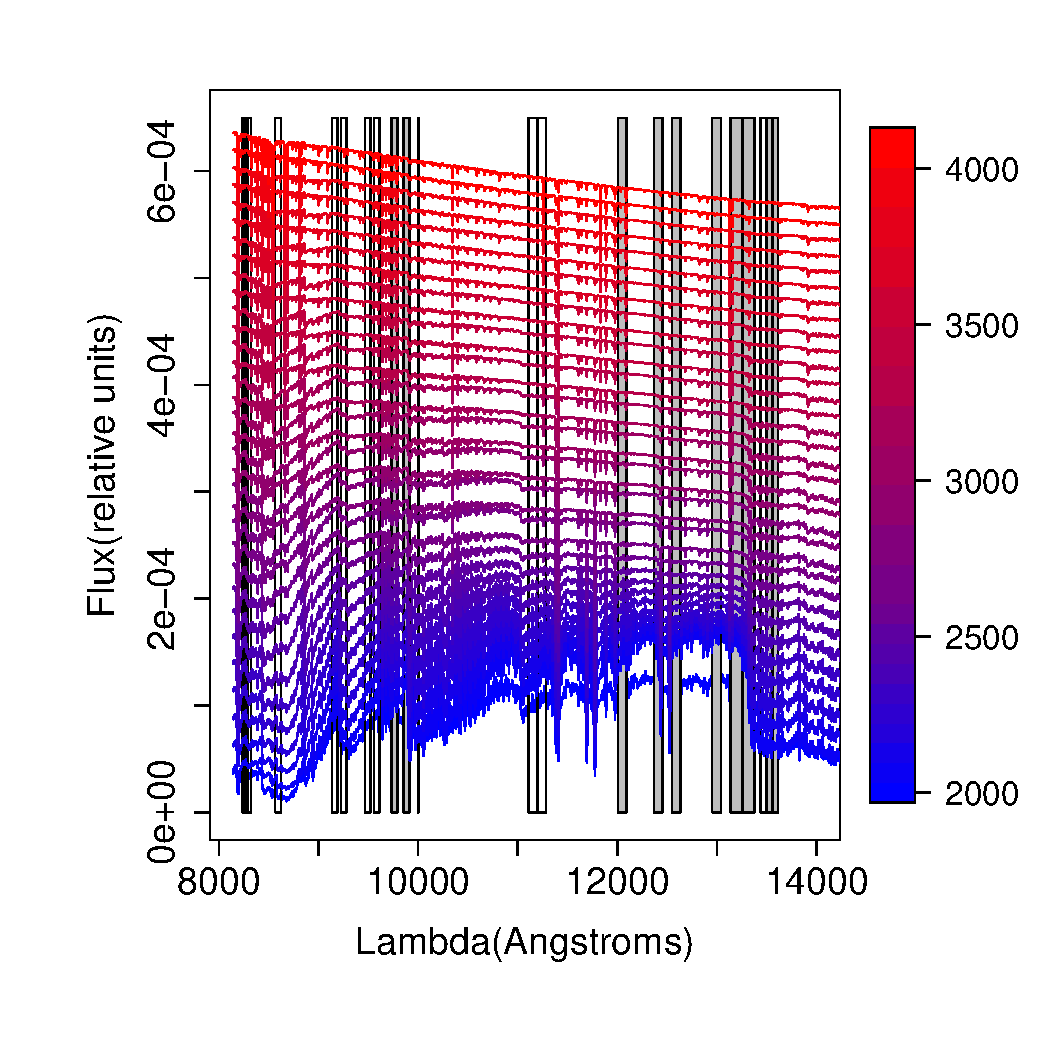
\includegraphics[scale=0.55]{figs/BT-spectraAtIRTF-Inf-teff}
  \caption{Features selected by the GA for predicting $T_{eff}$ using
    BT\_Settl noiseless synthetic spectra in the IRTF wavelength range
    and resolution. The BT\ Settl spectra are plot in a colour scale
    that ranges from blue (2000 K) to red (4100 K). The empty boxes
    correspond to the selected features and the grey boxes to the
    continuum bands.}
\label{fig:irtf-teff-inf}
\end {figure}


\begin{table*}
\begin{center}

  \begin{tabular}{rrrr | rrrr}
  \hline
 \multicolumn{4}{c}{SNR = 10} &  \multicolumn{4}{c}{SNR=50} \\
  \hline
$\lambda_1$ & $\lambda_2$ & $\lambda_{cont;1}$ & $\lambda_{cont;2} $ & $\lambda_1$ & $\lambda_2$ & $\lambda_{cont;1}$ & $\lambda_{cont;2} $ \\ 
  \hline
8235.96  & 8294.04   & 12681.62 & 12768.68   &  8145.92 & 8204.03   & 12636.48 & 12723.57 \\   
8505.89  & 8563.93   & 13378.12 & 13494.13   &  8895.95 & 8953.95   & 11331.57 & 11418.65 \\     
9376.07  & 9433.92   & 12951.62 & 13038.62   &  8176.03 & 8234.13   & 10611.36 & 10698.46 \\      
8145.92  & 8204.03   & 12366.32 & 12453.33   &  13438.08 & 13554.08 & 12546.46 & 12633.49 \\     
9195.86  & 9253.93   & 9135.89 & 9193.92     &  8235.96 & 8294.04   & 11961.44 & 12048.54 \\      
9585.95  & 9644.12   & 10002.04 & 9999.92    &  9376.07 & 9433.92   & 10002.04 & 9999.92  \\   
8385.99  & 8443.94   & 11826.48 & 11913.28   &  9406.09 & 9463.96   & 13258.32 & 13374.32 \\    
9135.89  & 9193.92   & 9225.86 & 9283.94     &  9346.13 & 9403.92   & 13086.46 & 13194.09 \\   
13618.20 & 13734.15  & 11376.63 & 11463.51   &  11106.48 & 11193.56 & 13438.08 & 13554.08 \\    
9105.87  & 9163.91   & 8865.98 & 8923.94     &  9255.86 & 9314.01   & 8865.98  & 8923.94  \\    
\hline
\end{tabular}
\caption {Recommended features and continuum bandpasses for predicting
  $ T_{eff} $ using BT\_Settl with SNR= $ 10 $ and 50 and the IRTF
  wavelength range and resolution.} \label{tab:irtf-teff-noisy}
\end{center}
\end{table*}

\begin {figure}
 \centering
  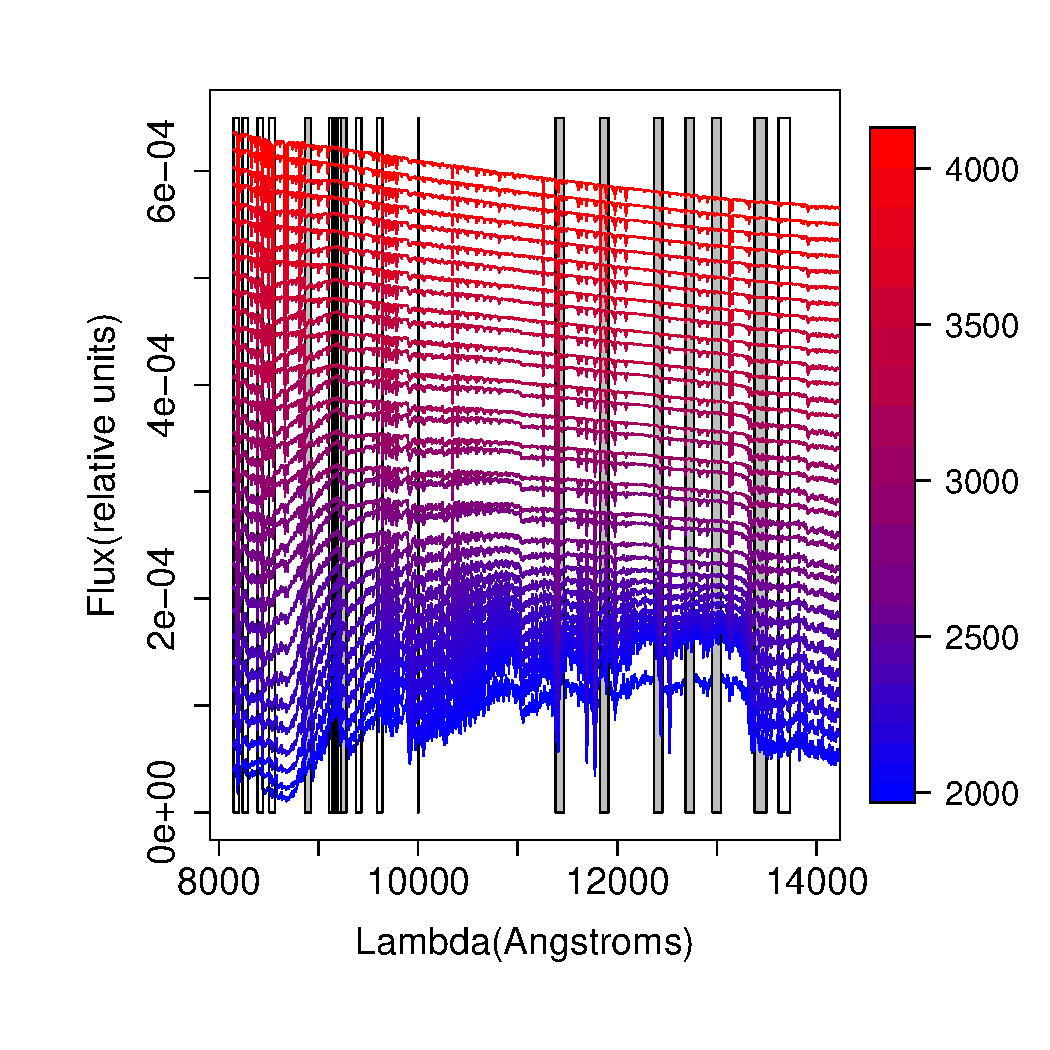
\includegraphics[scale=0.55]{figs/BT-spectraAtIRTF-10-teff}
  \caption{Features selected by the GA for predicting $T_{eff}$ using
    BT\_Settl synthetic spectra of SNR=10 in the IRTF wavelength range
    and resolution. The BT\ Settl spectra are plot in a colour scale
    that ranges from blue (2000 K) to red (4100 K). The empty boxes
    correspond to the selected features and the grey boxes to the
    continuum bands.}
\label{fig:irtf-teff-10}
\end {figure}

\begin {figure}
 \centering
  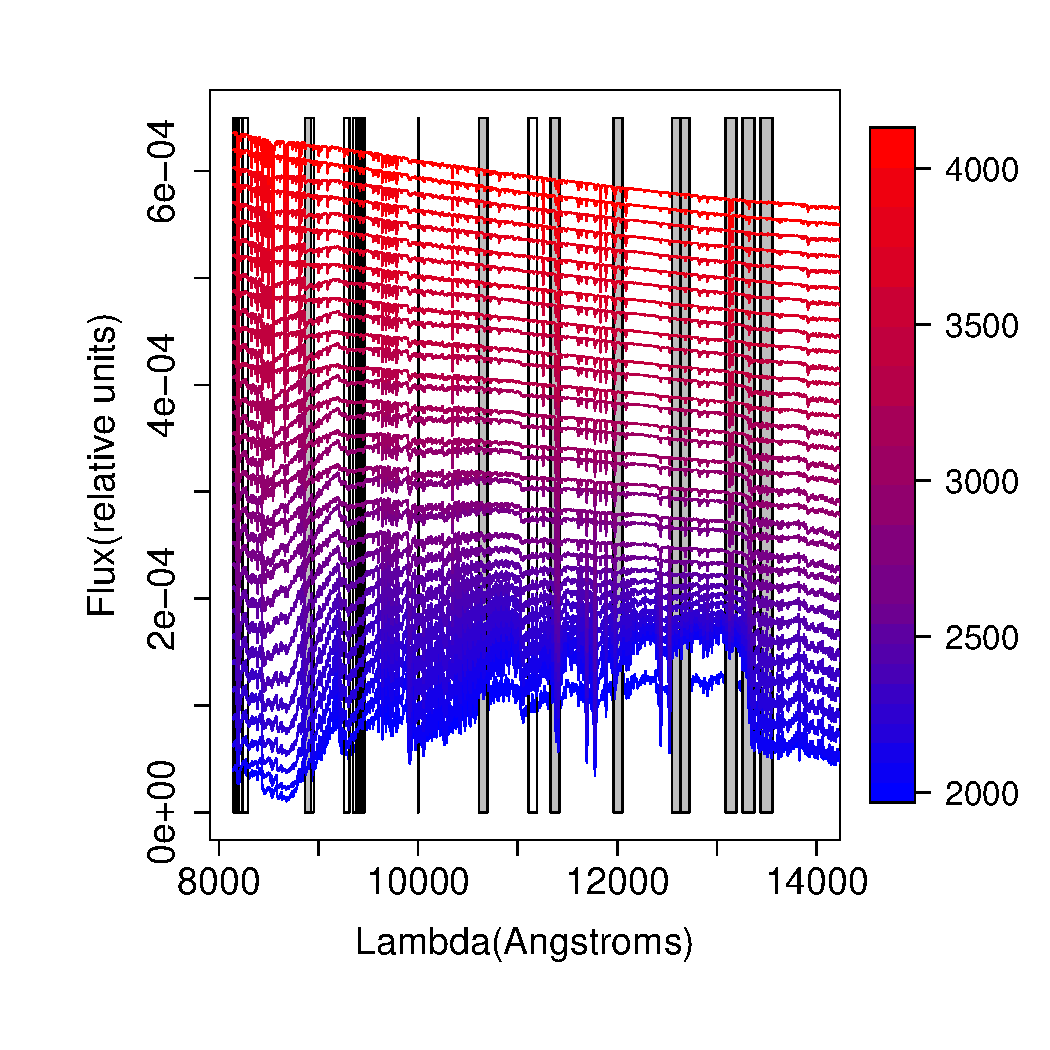
\includegraphics[scale=0.55]{figs/BT-spectraAtIRTF-50-teff}
  \caption{Features selected by the GA for predicting $T_{eff}$ using
    BT\_Settl synthetic spectra of SNR=50 in the IRTF wavelength range
    and resolution. The BT\ Settl spectra are plot in a colour scale
    that ranges from blue (2000 K) to red (4100 K). The empty boxes
    correspond to the selected features and the grey boxes to the
    continuum bands.}
\label{fig:irtf-teff-50}
\end {figure}


\begin{table*}
\begin{center}
\begin{tabular}{rrrrrrrr}
  \hline
Index & Element & Signal\_from & Signal\_To & Cont1\_From & Cont1\_To & Cont2\_From & Cont2\_To \\ 
  \hline
  Pa1 & H~{\sc i}   & 8461 & 8474 & 8474 & 8484 & 8563 & 8577 \\ 
  Ca1 & Ca~{\sc ii} & 8484 & 8513 & 8474 & 8484 & 8563 & 8577 \\ 
  Ca2 & Ca~{\sc ii} & 8522 & 8562  & 8474 & 8484 & 8563 & 8577 \\ 
  Pa2 & H~{\sc i}   & 8577 & 8619 & 8563 & 8577 & 8619 & 8642 \\ 
  Ca3 & Ca~{\sc ii} & 8642 & 8682 & 8619 & 8642 & 8700 & 8725 \\ 
  Pa3 & H~{\sc i}   & 8730 & 8772 & 8700 & 8725 & 8776 & 8792 \\ 
  Mg  & Mg~{\sc i}  & 8802 & 8811 & 8776 & 8792 & 8815 & 8850 \\ 
  Pa4 & H~{\sc i}   & 8850 & 8890 & 8815 & 8850 & 8890 & 8900 \\ 
  Pa5 & H~{\sc i}   & 9000 & 9030 & 8983 & 8998 & 9040 & 9050 \\
  FeClTi & Fe~{\sc i}, Cl~{\sc i}, Ti~{\sc i} &9080 & 9100 & 9040 & 9050 & 9125 & 9135 \\
  Pa6 & H~{\sc i}   &9217 & 9255 & 9152 & 9165 & 9265 & 9275 \\
Fe1         & Fe{~\sc i}     & 1.9297 & 1.9327~& 1.9220 & 1.9260 & 2.0030 & 2.0100 \\
Br$\delta$  & H{~\sc i} (n=4)& 1.9425 & 1.9470~& 1.9220 & 1.9260 & 2.0030 & 2.0100 \\
Ca1         & Ca{~\sc i}     & 1.9500 & 1.9526~& 1.9220 & 1.9260 & 2.0030 & 2.0100 \\
Fe23        & Fe{~\sc i}     & 1.9583 & 1.9656~& 1.9220 & 1.9260 & 2.0030 & 2.0100 \\
Si          & Si{~\sc i}     & 1.9708 & 1.9748~& 1.9220 & 1.9260 & 2.0030 & 2.0100 \\
Ca2         & Ca{~\sc i}     & 1.9769 & 1.9795~& 1.9220 & 1.9260 & 2.0030 & 2.0100 \\
Ca3         & Ca{~\sc i}     & 1.9847 & 1.9881~& 1.9220 & 1.9260 & 2.0030 & 2.0100 \\
Ca4         & Ca{~\sc i}     & 1.9917 & 1.9943~& 1.9220 & 1.9260 & 2.0030 & 2.0100 \\
Mg1         & Mg{~\sc i}     & 2.1040 & 2.1110~& 2.1000 & 2.1040 & 2.1110 & 2.1150 \\
Br$\gamma$  & H{~\sc i} (n=4)& 2.1639 & 2.1686~& 2.0907 & 2.0951 & 2.2873 & 2.2900 \\
Na$_{\rm d}$& Na{~\sc i}     & 2.2000 & 2.2140~& 2.1934 & 2.1996  & 2.2150 & 2.2190   \\
FeA         & Fe{~\sc i}     & 2.2250 & 2.2299~& 2.2133 & 2.2176 & 2.2437 & 2.2479 \\
FeB         & Fe{~\sc i}     & 2.2368 & 2.2414~& 2.2133 & 2.2176 & 2.2437 & 2.2479 \\
Ca$_{\rm d}$& Ca{~\sc i}     & 2.2594 & 2.2700~& 2.2516 & 2.2590  & 2.2716 & 2.2888   \\
Mg2         & Mg{~\sc i}     & 2.2795 & 2.2845~& 2.2700 & 2.2720 & 2.2850 & 2.2874 \\
$^{12}$CO   & $^{12}$CO(2,0) & 2.2910 & 2.3070~& 2.2516 & 2.2590   & 2.2716 & 2.2888   \\
\hline
\end{tabular}
\caption {Features and continuum bandpasses defined in 
   \protect\cite{cesetti} as relevant for the estimation of the
   effective temperature in bands I and K.} \label{tab:irtf-cesetti}
\end{center}
\end{table*}

% 1.2 logg

%
% Las tablas de features del GA para Teff están OK
% comprbadas el 2/11/2015 desde 
% http://apii01.etsii.upm.es:8787/files/git/M_prep_IRTF/prep_GA_case01_NG11F2_v1.html
% 
\begin{table}
\begin{center}
\begin{tabular}{rrrrrrr}
  \hline
  $\lambda_1$ & $\lambda_2$ & $\lambda_{cont;1}$ & $\lambda_{cont;2} $ \\ 
  \hline
     10245.88 & 10304.02 &	11241.29 & 11328.54 \\
     8415.91  & 8473.96  &	11511.51 & 11598.51\\
     12906.56 & 12993.61 &	13041.48 & 13133.82\\
     8716.00  & 8773.99  &	10425.90 & 10484.13\\
     8805.93  & 8863.97  &	12816.72 & 12903.73\\
     10126.02 & 10183.93 &	13086.46 & 13194.09\\
     8176.03  & 8234.13  &	10971.57 & 11058.46\\
     8626.02  & 8683.99  &	10746.43 & 10833.57\\
     8536.03  & 8594.06  &	10215.95 & 10274.10\\
     12951.62 & 13038.62 &	11196.56 & 11283.24 \\

\hline
\end{tabular}
\caption {Recommended features and continuum bandpasses for predicting
  $\log(g)$ using noiseless BT\_Settl spectra in the IRTF
  wavelength range and resolution.} \label{tab:irtf-logg-noiseless}
\end{center}
\end{table}

\begin {figure}
 \centering
  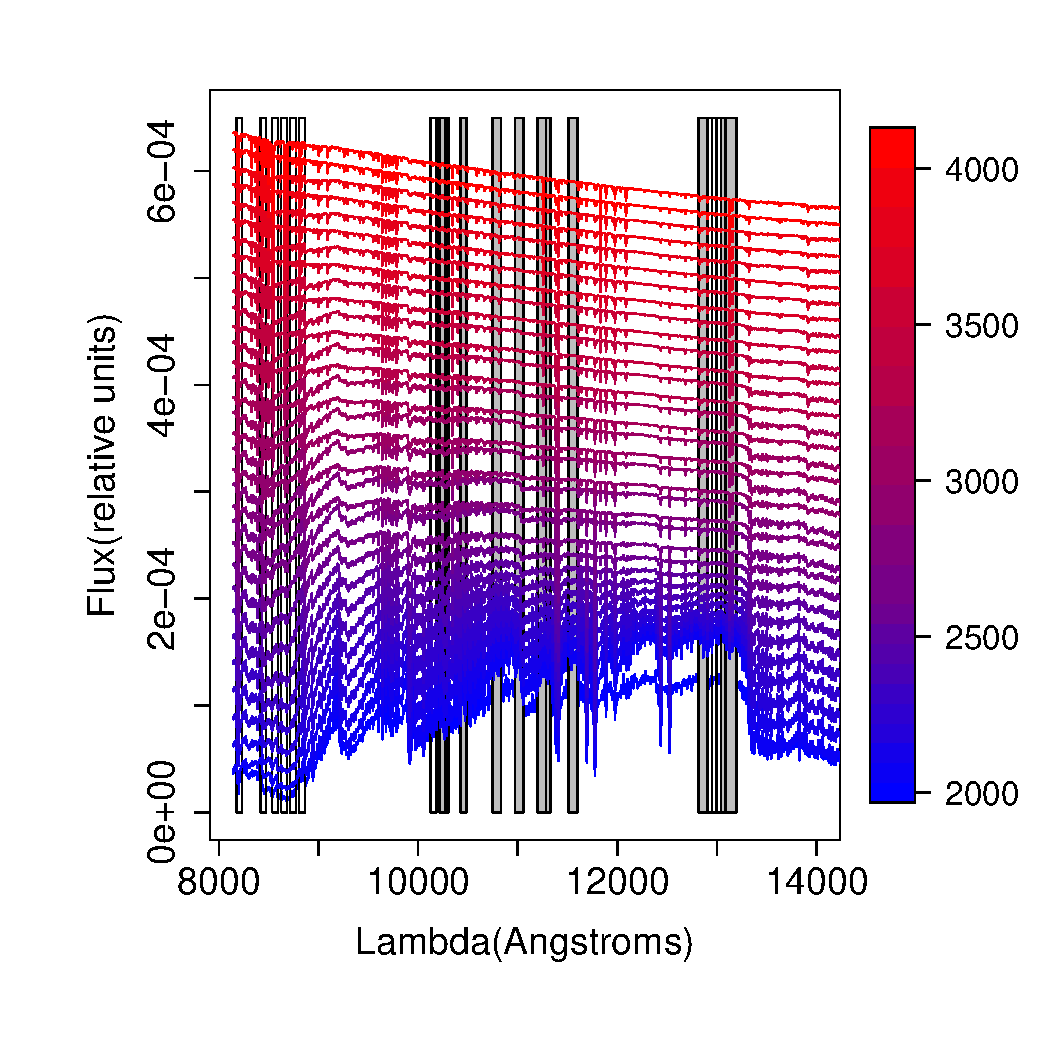
\includegraphics[scale=0.55]{figs/BT-spectraAtIRTF-Inf-logg}
  \caption{Features selected by the GA for predicting $\log(g)$ using
    BT\_Settl noiseless synthetic spectra in the IRTF wavelength range
    and resolution. The BT\ Settl spectra are plot in a colour scale
    that ranges from blue (2000 K) to red (4100 K). The empty boxes
    correspond to the selected features and the grey boxes to the
    continuum bands.}
\label{fig:irtf-logg-inf}
\end {figure}


\begin{table*}
\begin{center}
\begin{tabular}{rrrr | rrrr}
  \hline
 \multicolumn{4}{c}{SNR = 10} &  \multicolumn{4}{c}{SNR=50} \\
  \hline
$\lambda_1$ & $\lambda_2$ & $\lambda_{cont;1}$ & $\lambda_{cont;2} $ & $\lambda_1$ & $\lambda_2$ & $\lambda_{cont;1}$ & $\lambda_{cont;2} $ \\ 
  \hline
     8176.03  & 8234.13  &	9165.87  & 9223.91  &  11151.63 & 11238.46 &      13086.46 & 13194.09 \\
     10485.99 & 10563.41 &	10002.04 & 9999.92  &  8385.99  & 8443.94  &      13618.20 & 13734.14 \\
     8656.09  & 8714.047 &      10926.46 & 11013.60 &  8176.03  & 8234.13  &      11241.29 & 11328.54 \\
     9525.89  & 9584.059 &	10002.04 & 9999.92  &  8536.03  & 8594.06  &      13041.48 & 13133.82 \\ 
     8205.98  & 8263.967 &	13041.48 & 13133.82 &  12771.70 & 12858.73 &      10306.03 & 10363.88 \\
     10275.97 & 10333.96 &	11376.63 & 11463.51 &  13378.12 & 13494.13 &      10002.04 & 9999.92  \\
     10306.03 & 10363.88 &	11151.63 & 11238.46 &  8626.02  & 8683.99  &      10926.46 & 11013.60 \\
     9165.87  & 9223.91  &	8385.99  & 8443.94  &  9826.05  & 9883.91  &      10006.07 & 10064.01 \\
     9645.82  & 9704.16  &	13137.94 & 13253.96 &  10521.56 & 10608.46 &      11736.71 & 11823.49 \\
     8326.00  & 8383.94  &	12726.69 & 12813.71 &  8205.98  & 8263.96  &      9796.09  & 9853.94  \\ 
   \hline
\end{tabular}
\caption {Recommended features and continuum bandpasses for predicting
  $log(g)$ using BT-Settl spectra of SNR= $10$ and 50 in the IRTF
  wavelength range and resolution.} \label{tab:irtf-logg-noisy}
\end{center}
\end{table*}

\begin {figure}
 \centering
  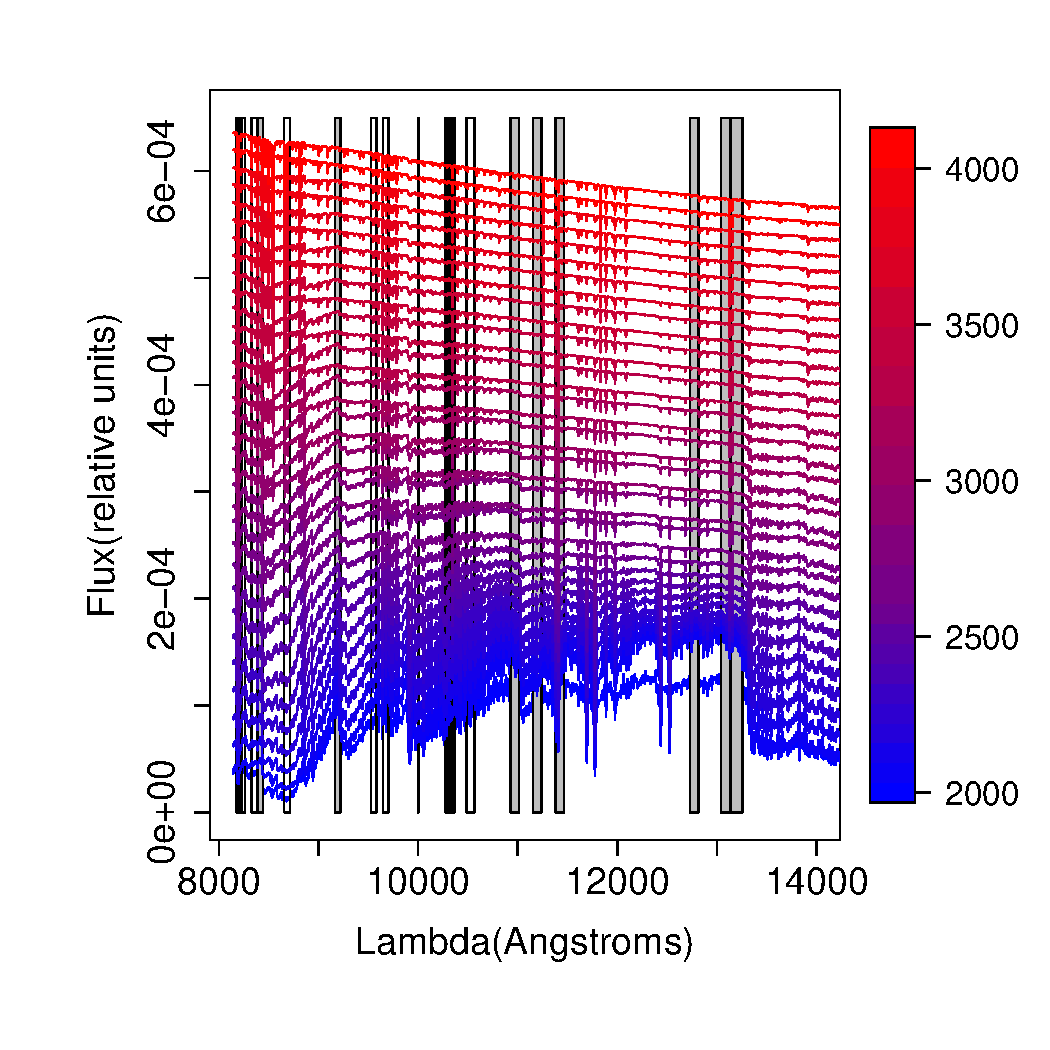
\includegraphics[scale=0.55]{figs/BT-spectraAtIRTF-10-logg}
  \caption{Features selected by the GA for predicting $\log(g)$ using
    BT\_Settl synthetic spectra of SNR=10 in the IRTF wavelength range
    and resolution. The BT\ Settl spectra are plot in a colour scale
    that ranges from blue (2000 K) to red (4100 K). The empty boxes
    correspond to the selected features and the grey boxes to the
    continuum bands.}
\label{fig:irtf-logg-10}
\end {figure}

\begin {figure}
 \centering
  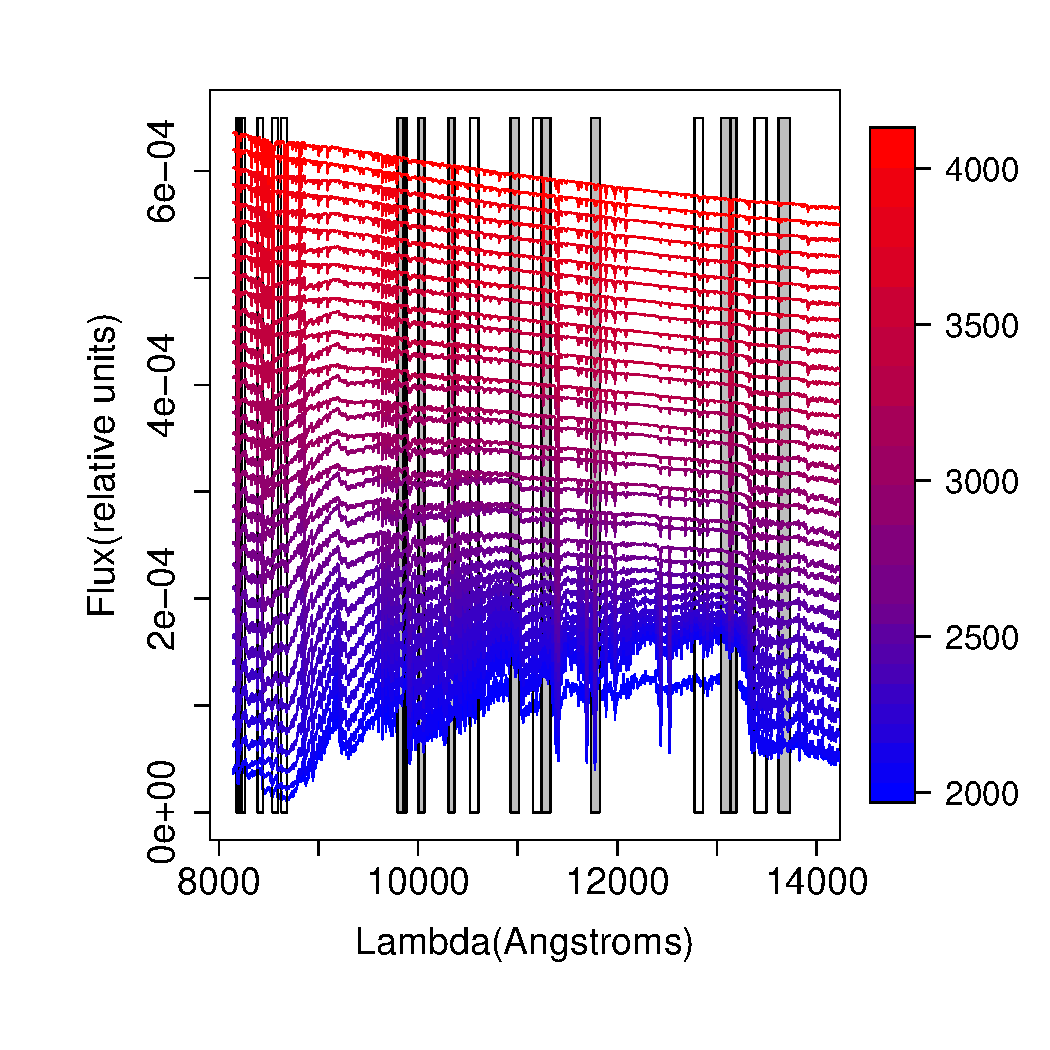
\includegraphics[scale=0.55]{figs/BT-spectraAtIRTF-50-logg}
  \caption{Features selected by the GA for predicting $\log(g)$ using
    BT\_Settl synthetic spectra of SNR=50 in the IRTF wavelength range
    and resolution. The BT\ Settl spectra are plot in a colour scale
    that ranges from blue (2000 K) to red (4100 K). The empty boxes
    correspond to the selected features and the grey boxes to the
    continuum bands.}
\label{fig:irtf-logg-50}
\end {figure}

% 1.3 Metallicity

%
% Las tablas de features del GA para Teff están OK
% comprbadas el 2/11/2015 desde 
% http://apii01.etsii.upm.es:8787/files/git/M_prep_IRTF/
% 
\begin{table}
\begin{center}
\begin{tabular}{rrrrrrr}
  \hline
  $\lambda_1$ & $\lambda_2$ & $\lambda_{cont;1}$ & $\lambda_{cont;2} $ \\ 
  \hline
     12096.68 & 12183.66  & 12051.50 & 12096.68 \\
     9525.89 & 9584.05 	  & 12321.33 & 12408.32 \\
     8205.98 & 8263.96 	  & 10126.02 & 10183.93 \\
     8566.08 & 8624.07 	  & 12276.52 & 12363.34 \\
     11196.56 & 11283.24  & 11151.63 & 11196.56 \\
     11151.639 & 11238.46 & 11466.35 & 11553.33 \\
     9555.93 & 9614.06 	  & 8205.98  & 8263.96 \\
     11016.62 & 11103.37  & 10791.44 & 10878.40 \\
     9766.16 & 9823.94 	  & 12681.62 & 12768.68 \\
     9942.14 & 9999.92   & 9555.93  & 9614.06 \\
\hline
\end{tabular}
\caption {Feature and Continuum bandpasses selected for predicting
  metallicity using noiseless BT\_Settl spectra in the IRTF wavelength
  range and resolution.} \label{tab:irtf-met-noiseless}
\end{center}
\end{table}

\begin {figure}
 \centering
  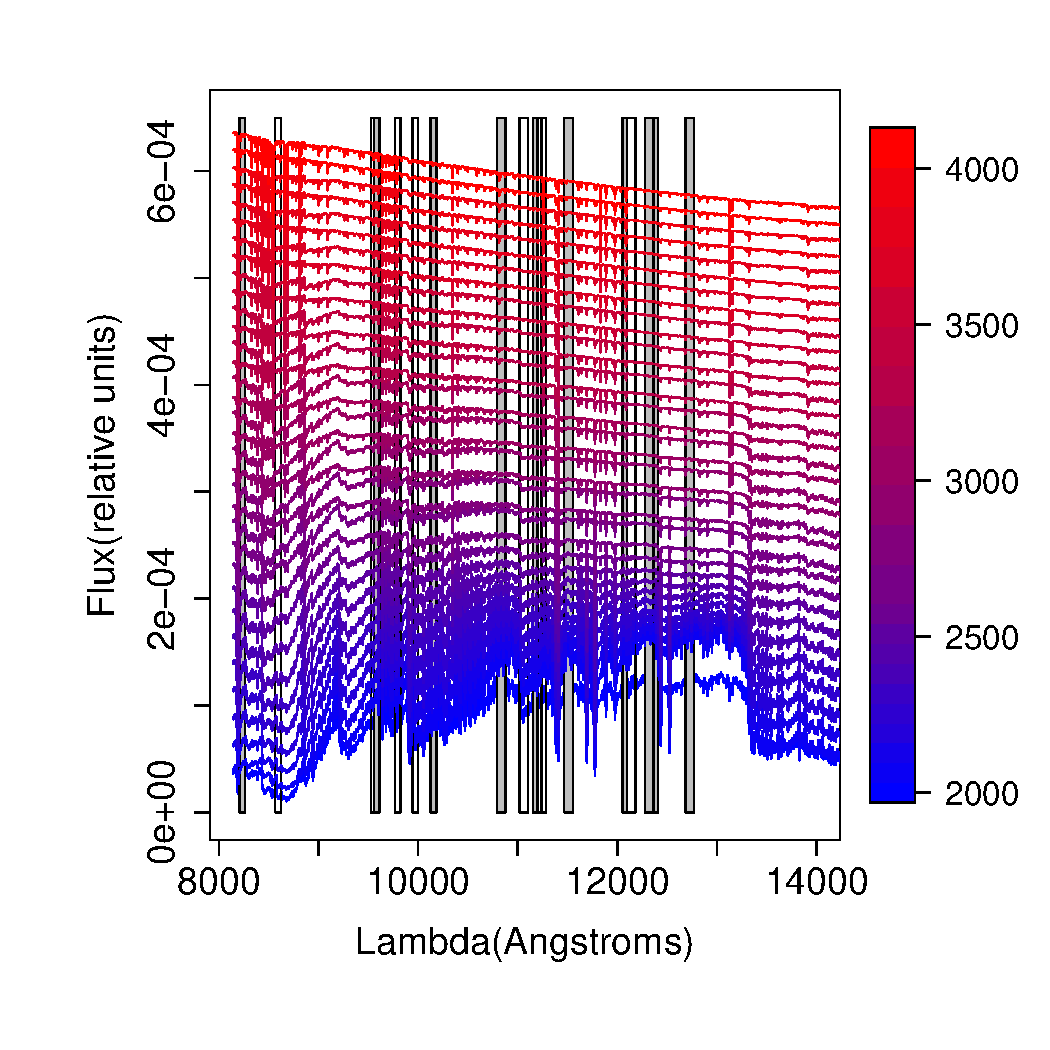
\includegraphics[scale=0.55]{figs/BT-spectraAtIRTF-Inf-mh}
  \caption{Features selected by the GA for predicting [M/H] using
    BT\_Settl noiseless synthetic spectra in the IRTF wavelength range
    and resolution. The BT\ Settl spectra are plot in a colour scale
    that ranges from blue (2000 K) to red (4100 K). The empty boxes
    correspond to the selected features and the grey boxes to the
    continuum bands.}
\label{fig:irtf-met-inf}
\end {figure}


\begin{table*}
\begin{center}
\begin{tabular}{rrrr | rrrr}
  \hline
 \multicolumn{4}{c}{SNR = 10} &  \multicolumn{4}{c}{SNR=50} \\
  \hline
$\lambda_1$ & $\lambda_2$ & $\lambda_{cont;1}$ & $\lambda_{cont;2} $ & $\lambda_1$ & $\lambda_2$ & $\lambda_{cont;1}$ & $\lambda_{cont;2} $ \\ 
  \hline

8235.96  & 8294.04  &	11331.57 & 11418.65 & 9255.86 & 9314.01   &     13197.94 & 13313.92  \\
9376.07  & 9433.92  &	10566.33 & 10653.62 & 8385.99 & 8443.94   &     9376.07  & 9433.92    \\
10306.03 & 10363.88 &	 9942.14 & 9999.92  & 8716.00 & 8773.99   &     9585.95  & 9644.12    \\
11286.42 & 11373.45 &	11241.29 & 11286.42 & 8235.96 & 8294.04   &     13086.46 & 13194.09  \\
9676.00  & 9734.02  &	13086.46 & 13194.09 & 9676.00 & 9734.02   &     10791.44 & 10878.40  \\
8775.95  & 8833.94  &	8415.91  & 8473.96  & 8415.91 & 8473.96   &     12411.34 & 12498.41  \\
12411.34 & 12498.41 &	10245.88 & 10304.02 & 8446.03 & 8503.94   &     9406.09  & 9463.96    \\
8476.01  & 8534.03  &	12276.52 & 12363.34 & 8205.98 & 8263.96   &     8955.88  & 9013.95    \\
12636.48 & 12723.57 &	12051.50 & 12138.72 & 8985.93 & 9043.98   &     12186.62 & 12273.48  \\
8415.91  & 8473.96  &	13618.20 & 13734.14 & 9015.98 & 9073.98   &     11241.29 & 11328.54  \\

\hline
\end{tabular}
\caption {Feature and Continuum bandpasses selected for predicting metallicity 
      using noisy BT\_Settl spectra with signal-to-noise ratios
      equal to 10 and 50 in the IRTF wavelength range
  and resolution.} \label{tab:irtf-met-noisy}
\end{center}
\end{table*}

\begin {figure}
 \centering
  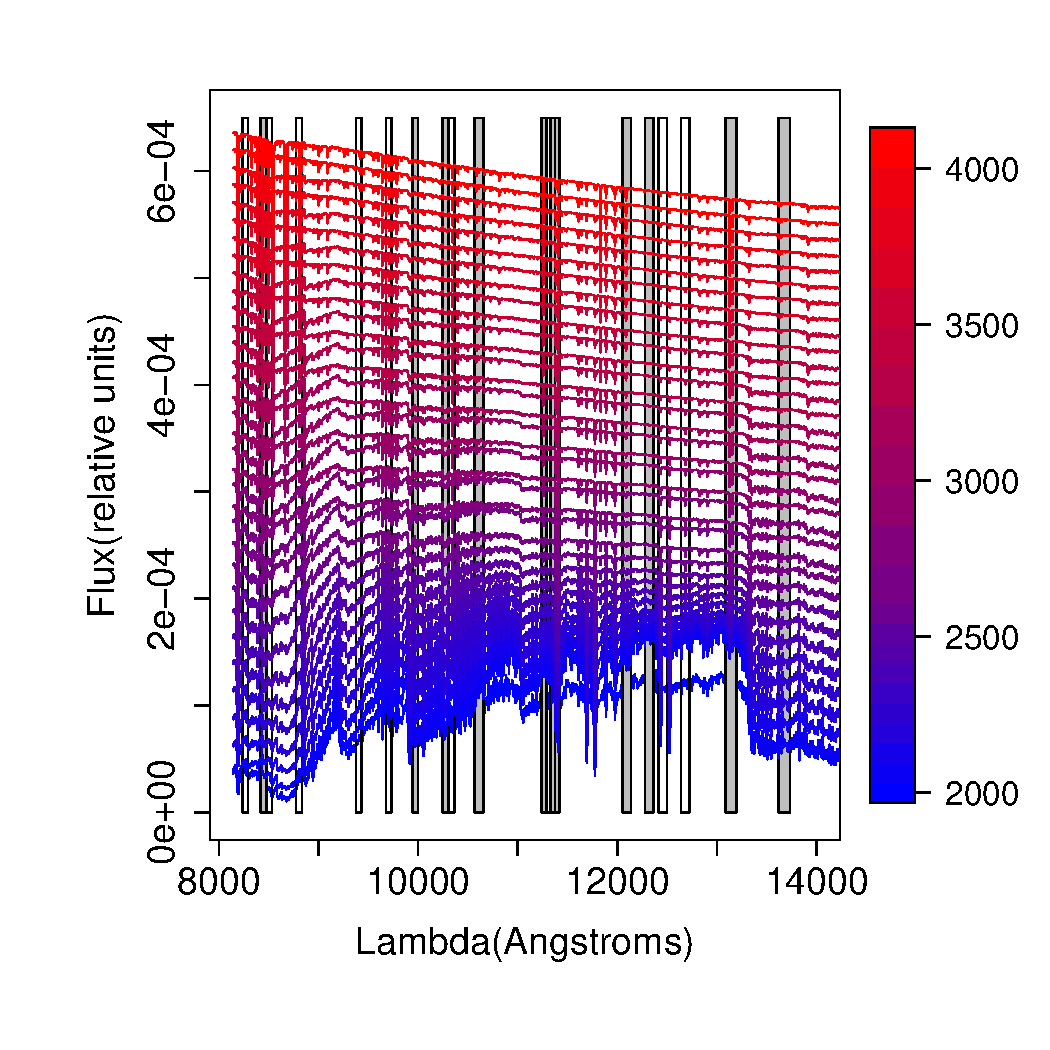
\includegraphics[scale=0.55]{figs/BT-spectraAtIRTF-10-mh}
  \caption{Features selected by the GA for predicting [M/H] using
    BT\_Settl synthetic spectra of SNR=10 in the IRTF wavelength range
    and resolution. The BT\ Settl spectra are plot in a colour scale
    that ranges from blue (2000 K) to red (4100 K). The empty boxes
    correspond to the selected features and the grey boxes to the
    continuum bands.}
\label{fig:irtf-met-10}
\end {figure}

\begin {figure}
 \centering
  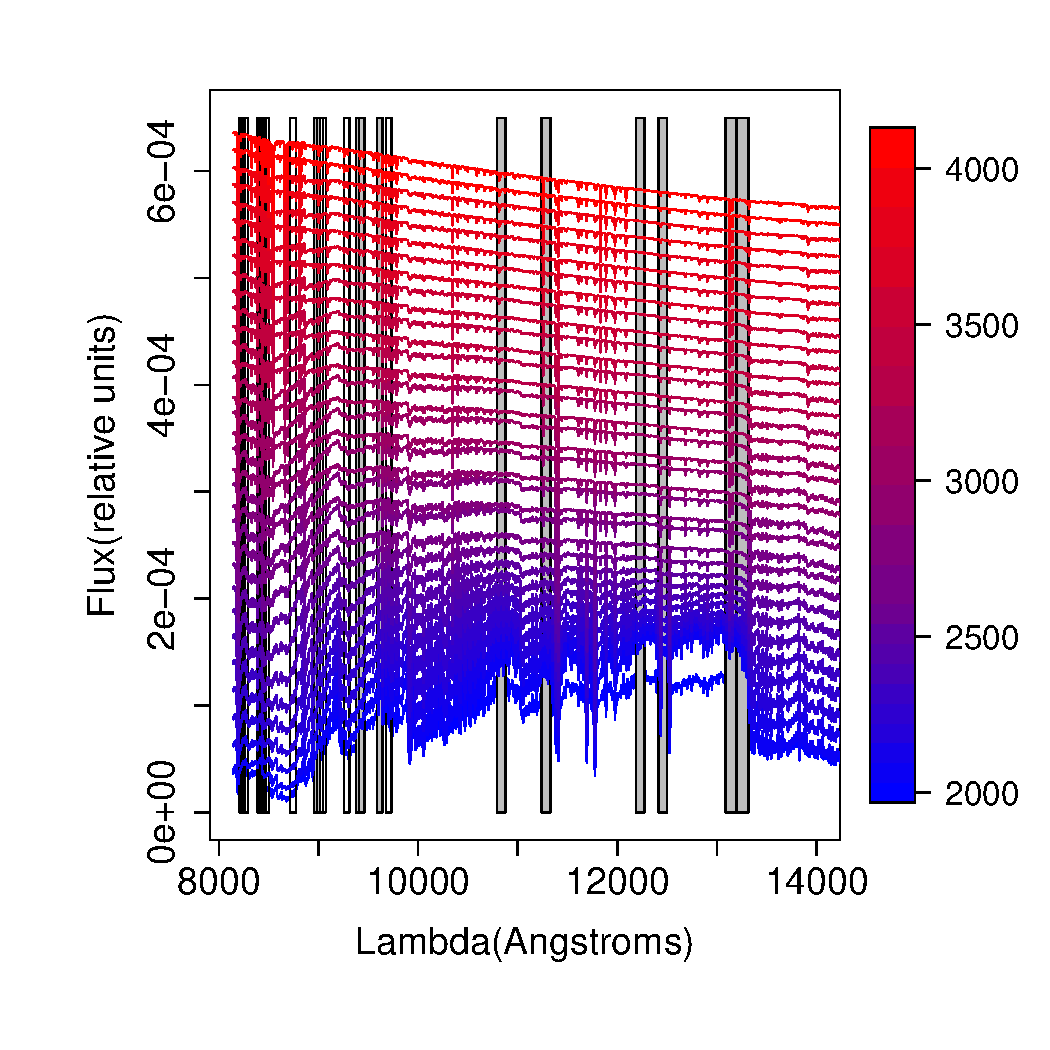
\includegraphics[scale=0.55]{figs/BT-spectraAtIRTF-50-mh}
  \caption{Features selected by the GA for predicting [M/H] using
    BT\_Settl synthetic spectra of SNR=50 in the IRTF wavelength range
    and resolution. The BT\ Settl spectra are plot in a colour scale
    that ranges from blue (2000 K) to red (4100 K). The empty boxes
    correspond to the selected features and the grey boxes to the
    continuum bands.}
\label{fig:irtf-met-50}
\end {figure}

\section{IPAC features}
\label{app:features:ipac}

% 2 IPAC

% 2.1 Teff


\begin{table}
\begin{center}
\begin{tabular}{rrrr}
  \hline
  $\lambda_1$ & $\lambda_2$ & $\lambda_{cont;1}$ & $\lambda_{cont;2} $ \\ 
  \hline 
  
7062 & 7094.4 &	7314 & 7346.4 \\
7116 & 7148.4 &	7782 & 7814.4 \\
7134 & 7166.4 &	7872 & 7904.4 \\
6900 & 6932.4 &	7764 & 7796.4 \\
7170 & 7202.4 &	7890 & 7922.4 \\
7080 & 7112.4 &	7926 & 7958.4 \\
7188 & 7220.4 &	7548 & 7580.4 \\
7800 & 7832.4 &	7962 & 7994.4 \\
6990 & 7022.4 &	7008 & 7040.4 \\
7026 & 7058.4 &	6990 & 7022.4 \\

\hline
\end{tabular}
\caption {Spectral features and continuum bandpasses selected by the
  GA for predicting $T_{\rm eff}$ using noiseless BT\_Settl spectra in
  the IPAC wavelength range and
  resolution.} \label{tab:ipac-teff-noiseless}
\end{center}
\end{table}


\begin{table*}
\begin{center}
\begin{tabular}{rrrr | rrrr}
  \hline
 \multicolumn{4}{c}{SNR = 10} &  \multicolumn{4}{c}{SNR=50} \\
  \hline
$\lambda_1$ & $\lambda_2$ & $\lambda_{cont;1}$ & $\lambda_{cont;2} $ & $\lambda_1$ & $\lambda_2$ & $\lambda_{cont;1}$ & $\lambda_{cont;2} $ \\ 
  \hline
7692 & 7724.4 	6936 & 6968.4  & 7062 & 7094.4 &  7296 & 7328.4 \\
6990 & 7022.4 	7998 & 8030.4  & 7026 & 7058.4 &  7044 & 7076.4 \\
6900 & 6932.4 	7548 & 7580.4  & 7080 & 7112.4 &  7926 & 7958.4 \\
7854 & 7886.4 	7710 & 7742.4  & 6900 & 6932.4 &  7548 & 7580.4 \\
7116 & 7148.4 	7908 & 7940.4  & 7134 & 7166.4 &  7836 & 7868.4 \\
7278 & 7310.4 	7926 & 7958.4  & 7296 & 7328.4 &  7962 & 7994.4 \\
7152 & 7184.4 	7746 & 7778.4  & 6936 & 6968.4 &  7728 & 7760.4 \\
7134 & 7166.4 	7764 & 7796.4  & 6972 & 7004.4 &  6900 & 6932.4 \\
6918 & 6950.4 	6900 & 6932.4  & 6990 & 7022.4 &  7944 & 7976.4 \\
7224 & 7256.4 	7962 & 7994.4  & 6918 & 6950.4 &  7782 & 7814.4 \\

\hline
\end{tabular}
\caption {Spectral features and continuum bandpasses selected by the
  GA for predicting $ T_{eff}$ using BT\_Settl spectra with SNR=10 and
  50 in the IPAC wavelength range and
  resolution.} \label{tab:ipac-teff-noisy}
\end{center}
\end{table*}

% 2.2 logg

\begin{table}
\begin{center}
\begin{tabular}{rrrr}
  \hline
  $\lambda_1$ & $\lambda_2$ & $\lambda_{cont;1}$ & $\lambda_{cont;2} $ \\ 
  \hline

7134 & 7166.4 &	7044 & 7076.4 \\
6954 & 6986.4 &	7152 & 7184.4 \\
7512 & 7544.4 &	7890 & 7922.4 \\
7062 & 7094.4 &	7224 & 7256.4 \\
6936 & 6968.4 &	7854 & 7886.4 \\
6900 & 6932.4 &	7746 & 7778.4 \\
6918 & 6950.4 &	7800 & 7832.4 \\
7008 & 7040.4 &	7134 & 7166.4 \\
7872 & 7904.4 &	7008 & 7040.4 \\
7962 & 7994.4 &	7980 & 8012.4 \\

\hline
\end{tabular}
\caption {Spectral features and continuum bandpasses selected by the
  GA for predicting $\log(g)$ using noiseless BT\_Settl spectra in the
  IPAC wavelength range and resolution..} \label{tab:ipac-logg-noiseless}
\end{center}
\end{table}

\begin{table*}
\begin{center}
\begin{tabular}{rrrr | rrrr}
  \hline
 \multicolumn{4}{c}{SNR = 10} &  \multicolumn{4}{c}{SNR=50} \\
  \hline
$\lambda_1$ & $\lambda_2$ & $\lambda_{cont;1}$ & $\lambda_{cont;2} $ & $\lambda_1$ & $\lambda_2$ & $\lambda_{cont;1}$ & $\lambda_{cont;2} $ \\ 
  \hline

6990 & 7022.4 &	6918 & 6950.4 & 6918 & 6950.4 & 6936 & 6968.4  \\
6900 & 6932.4 &	7278 & 7310.4 & 6936 & 6968.4 & 7836 & 7868.4  \\
7062 & 7094.4 &	7242 & 7274.4 & 7656 & 7688.4 & 7890 & 7922.4  \\
7692 & 7724.4 &	7008 & 7040.4 & 6900 & 6932.4 & 7872 & 7904.4  \\
7656 & 7688.4 &	7998 & 8030.4 & 7008 & 7040.4 & 7044 & 7076.4  \\
6936 & 6968.4 &	7836 & 7868.4 & 7512 & 7544.4 & 7656 & 7688.4  \\
7206 & 7238.4 &	7062 & 7094.4 & 7440 & 7472.4 & 7332 & 7364.4  \\
7512 & 7544.4 &	7926 & 7958.4 & 7800 & 7832.4 & 7692 & 7724.4  \\
7764 & 7796.4 &	7710 & 7742.4 & 7404 & 7436.4 & 7548 & 7580.4  \\
7404 & 7436.4 &	7548 & 7580.4 & 7080 & 7112.4 & 7152 & 7184.4  \\
   \hline
\end{tabular}
\caption {Spectral features and continuum bandpasses selected by the
  GA for predicting $\log(g)$ using BT\_Settl spectra of SNR=10 and 50
  in the IPAC wavelength range and
  resolution.} \label{tab:ipac-logg-noisy}
\end{center}
\end{table*}

% 2.3 Metallicity

\begin{table}
\begin{center}
\begin{tabular}{rrrr}
  \hline
  $\lambda_1$ & $\lambda_2$ & $\lambda_{cont;1}$ & $\lambda_{cont;2} $ \\ 
  \hline
7188 & 7220.4 &	7854 & 7886.4 \\ 
7080 & 7112.4 &	7926 & 7958.4 \\
7116 & 7148.4 &	7098 & 7130.4 \\
7422 & 7454.4 &	7836 & 7868.4 \\
7350 & 7382.4 &	7998 & 8030.4 \\
7224 & 7256.4 &	7818 & 7850.4 \\
7710 & 7742.4 &	7062 & 7094.4 \\
7476 & 7508.4 &	7944 & 7976.4 \\
7134 & 7166.4 &	7584 & 7616.4 \\
7836 & 7868.4 &	7278 & 7310.4 \\
\hline
\end{tabular}
\caption {Spectral features and continuum bandpasses selected by the
  GA for predicting metallicity using noiseless BT\_Settl spectra in
  the IPAC wavelength range and resolution.} \label{tab:ipac-met-noiseless}
\end{center}
\end{table}

\begin{table*}
\begin{center}
\begin{tabular}{rrrr | rrrr}
  \hline
 \multicolumn{4}{c}{SNR = 10} &  \multicolumn{4}{c}{SNR=50} \\
  \hline
$\lambda_1$ & $\lambda_2$ & $\lambda_{cont;1}$ & $\lambda_{cont;2} $ & $\lambda_1$ & $\lambda_2$ & $\lambda_{cont;1}$ & $\lambda_{cont;2} $ \\ 
  \hline
7692 & 7724.4 &	7026 & 7058.4  &  7098 & 7130.4 & 7926 & 7958.4 \\
6900 & 6932.4 &	7008 & 7040.4  &  7188 & 7220.4 & 7962 & 7994.4  \\
7350 & 7382.4 &	7908 & 7940.4  &  7368 & 7400.4 & 7980 & 8012.4  \\
6918 & 6950.4 &	6900 & 6932.4  &  7116 & 7148.4 & 7872 & 7904.4  \\
7098 & 7130.4 &	7314 & 7346.4  &  7062 & 7094.4 & 7206 & 7238.4  \\
7440 & 7472.4 &	7872 & 7904.4  &  7584 & 7616.4 & 7170 & 7202.4  \\
7134 & 7166.4 &	7962 & 7994.4  &  6936 & 6968.4 & 6918 & 6950.4  \\
7368 & 7400.4 &	7926 & 7958.4  &  7692 & 7724.4 & 7890 & 7922.4  \\
7080 & 7112.4 &	7044 & 7076.4  &  7134 & 7166.4 & 7548 & 7580.4  \\
7044 & 7076.4 &	7980 & 8012.4  &  7494 & 7526.4 & 7998 & 8030.4  \\
\hline
\end{tabular}
\caption {Spectral features and continuum bandpasses selected by the
  GA for predicting metallicities using BT\_Settl spectra of SNR=10
  and 50 in the IPAC wavelength range and
  resolution.} \label{tab:ipac-met-noisy}
\end{center}
\end{table*}

